%------------------------------%
%% ✎ Dylan (V1) %%%%%%%%% ✅ %%
%% ✎ Alain (V2) %%%%%%%%% ✅ %%
%% ✎ Dylan (V3) %%%%%%%%% ✅ %%
%------------------------------%

% ACKNOWLEDGEMENTS
    \cleardoublepage
    \needspace{1\baselineskip} % Reserve space
\chapter*{Acknowledgements
    \label{body:remerciements}
    }
    \markboth{Acknowledgements}{}
    \markright{Preface}{}
    \addcontentsline{toc}{part}{Acknowledgements}

    % Introduction
\lettrine[lines=3, findent=8pt, nindent=0pt]{\lettrinefont W}{elcome} aboard this \textsl{collective} work. This adjective, in my eyes, best describes the genesis of this doctoral research, the result of four or five years – the exact count still escapes me – of shared labor. Similar to the construction of a house, however modest it may be in the urban landscape, this manuscript is the realization of the investment of many hands. This doctoral thesis, encompassing the manuscript and the scientific productions that stem from it, was made possible thanks to the contribution of many knowledge artisans. To these collaborators, true builders both intellectually and emotionally, to whom I wish to pay tribute, I fear I cannot name all of them within the limited space of these few pages. Nevertheless, I engage in this exercise of recognition, for which words alone would not suffice to fully express my gratitude. In this spirit, mindful of not being able to fully communicate my esteem for your support and daily efforts, I have chosen to materialize these acknowledgements in the form of a map (see the \hyperref[fig-introduction:remerciements]{Acknowledgement Map}, page~\pageref{fig-introduction:remerciements}). The first, but certainly not the last in this document, rest assured.%%Translated%%

    % Supervision
There can be no \textsl{correct} order to mention all the people who contributed to enriching this doctoral experience. However, I must first and foremost express my deepest gratitude to \textcolor{blue}{Alain L'Hostis}, who has exercised his responsibilities as thesis supervisor with constant kindness and good humor. His qualities, both scientific and human, have been an invaluable source of inspiration and encouragement throughout this journey. From my research internship, he welcomed me under the best conditions. I am deeply grateful to him for his availability, and especially for the trust and great freedom he granted me in guiding this project. This trust honors me, and I hope that this thesis, in its own way, manages to repay a part of what has been so generously given to me.%%Translated%%

    % CSI and Jury
I also wish to express my gratitude to \textcolor{blue}{Laurent Chapelon} and \textcolor{blue}{Chia-Lin Chen}, who evaluated this doctoral thesis as \textsl{rapporteurs}, as well as to \textcolor{blue}{Ahad Amini Pishro}, \textcolor{blue}{Sophie Hasiak}, and \textcolor{blue}{Patrick Rérat}, who agreed to be part of the jury. Furthermore, I extend my thanks to \textcolor{blue}{Marc Dumont} and \textcolor{blue}{Vaclav Stransky}, who generously accepted to follow the progress of my doctoral research. Lastly, my gratitude goes to \textcolor{blue}{Philippe Menerault}, whose teachings during my academic journey inspired me. His wise advice has been of invaluable help.%%Translated%%

    % Institutions
I am aware of the extremely favorable conditions under which my research was carried out, both in terms of financial support and scientific guidance. More broadly, I recognize the privilege of having worked in such a rich professional environment, both in Lille and in Paris, as part of a laboratory driven by such passionate and caring individuals. I owe this pleasant atmosphere largely to the support of Gustave Eiffel University and the Hauts-de-France Region, through the \textsl{rev3} program, which financed this research project.%%Translated%%

    % Support
\textsl{Last but not least}, it is impossible for me to continue writing this section dedicated to acknowledgements without mentioning my family, to whom I dedicate this manuscript. You are my role model, and I am committed to honoring the tenacity and ethical values you have passed on to me. To everyone I hold dear.%%Translated%%

    % Acknowledgement Map
    \begin{carte}[h!]\vspace*{4pt}
        \caption*{Acknowledgement Map}
        \label{fig-introduction:remerciements}
        \centerline{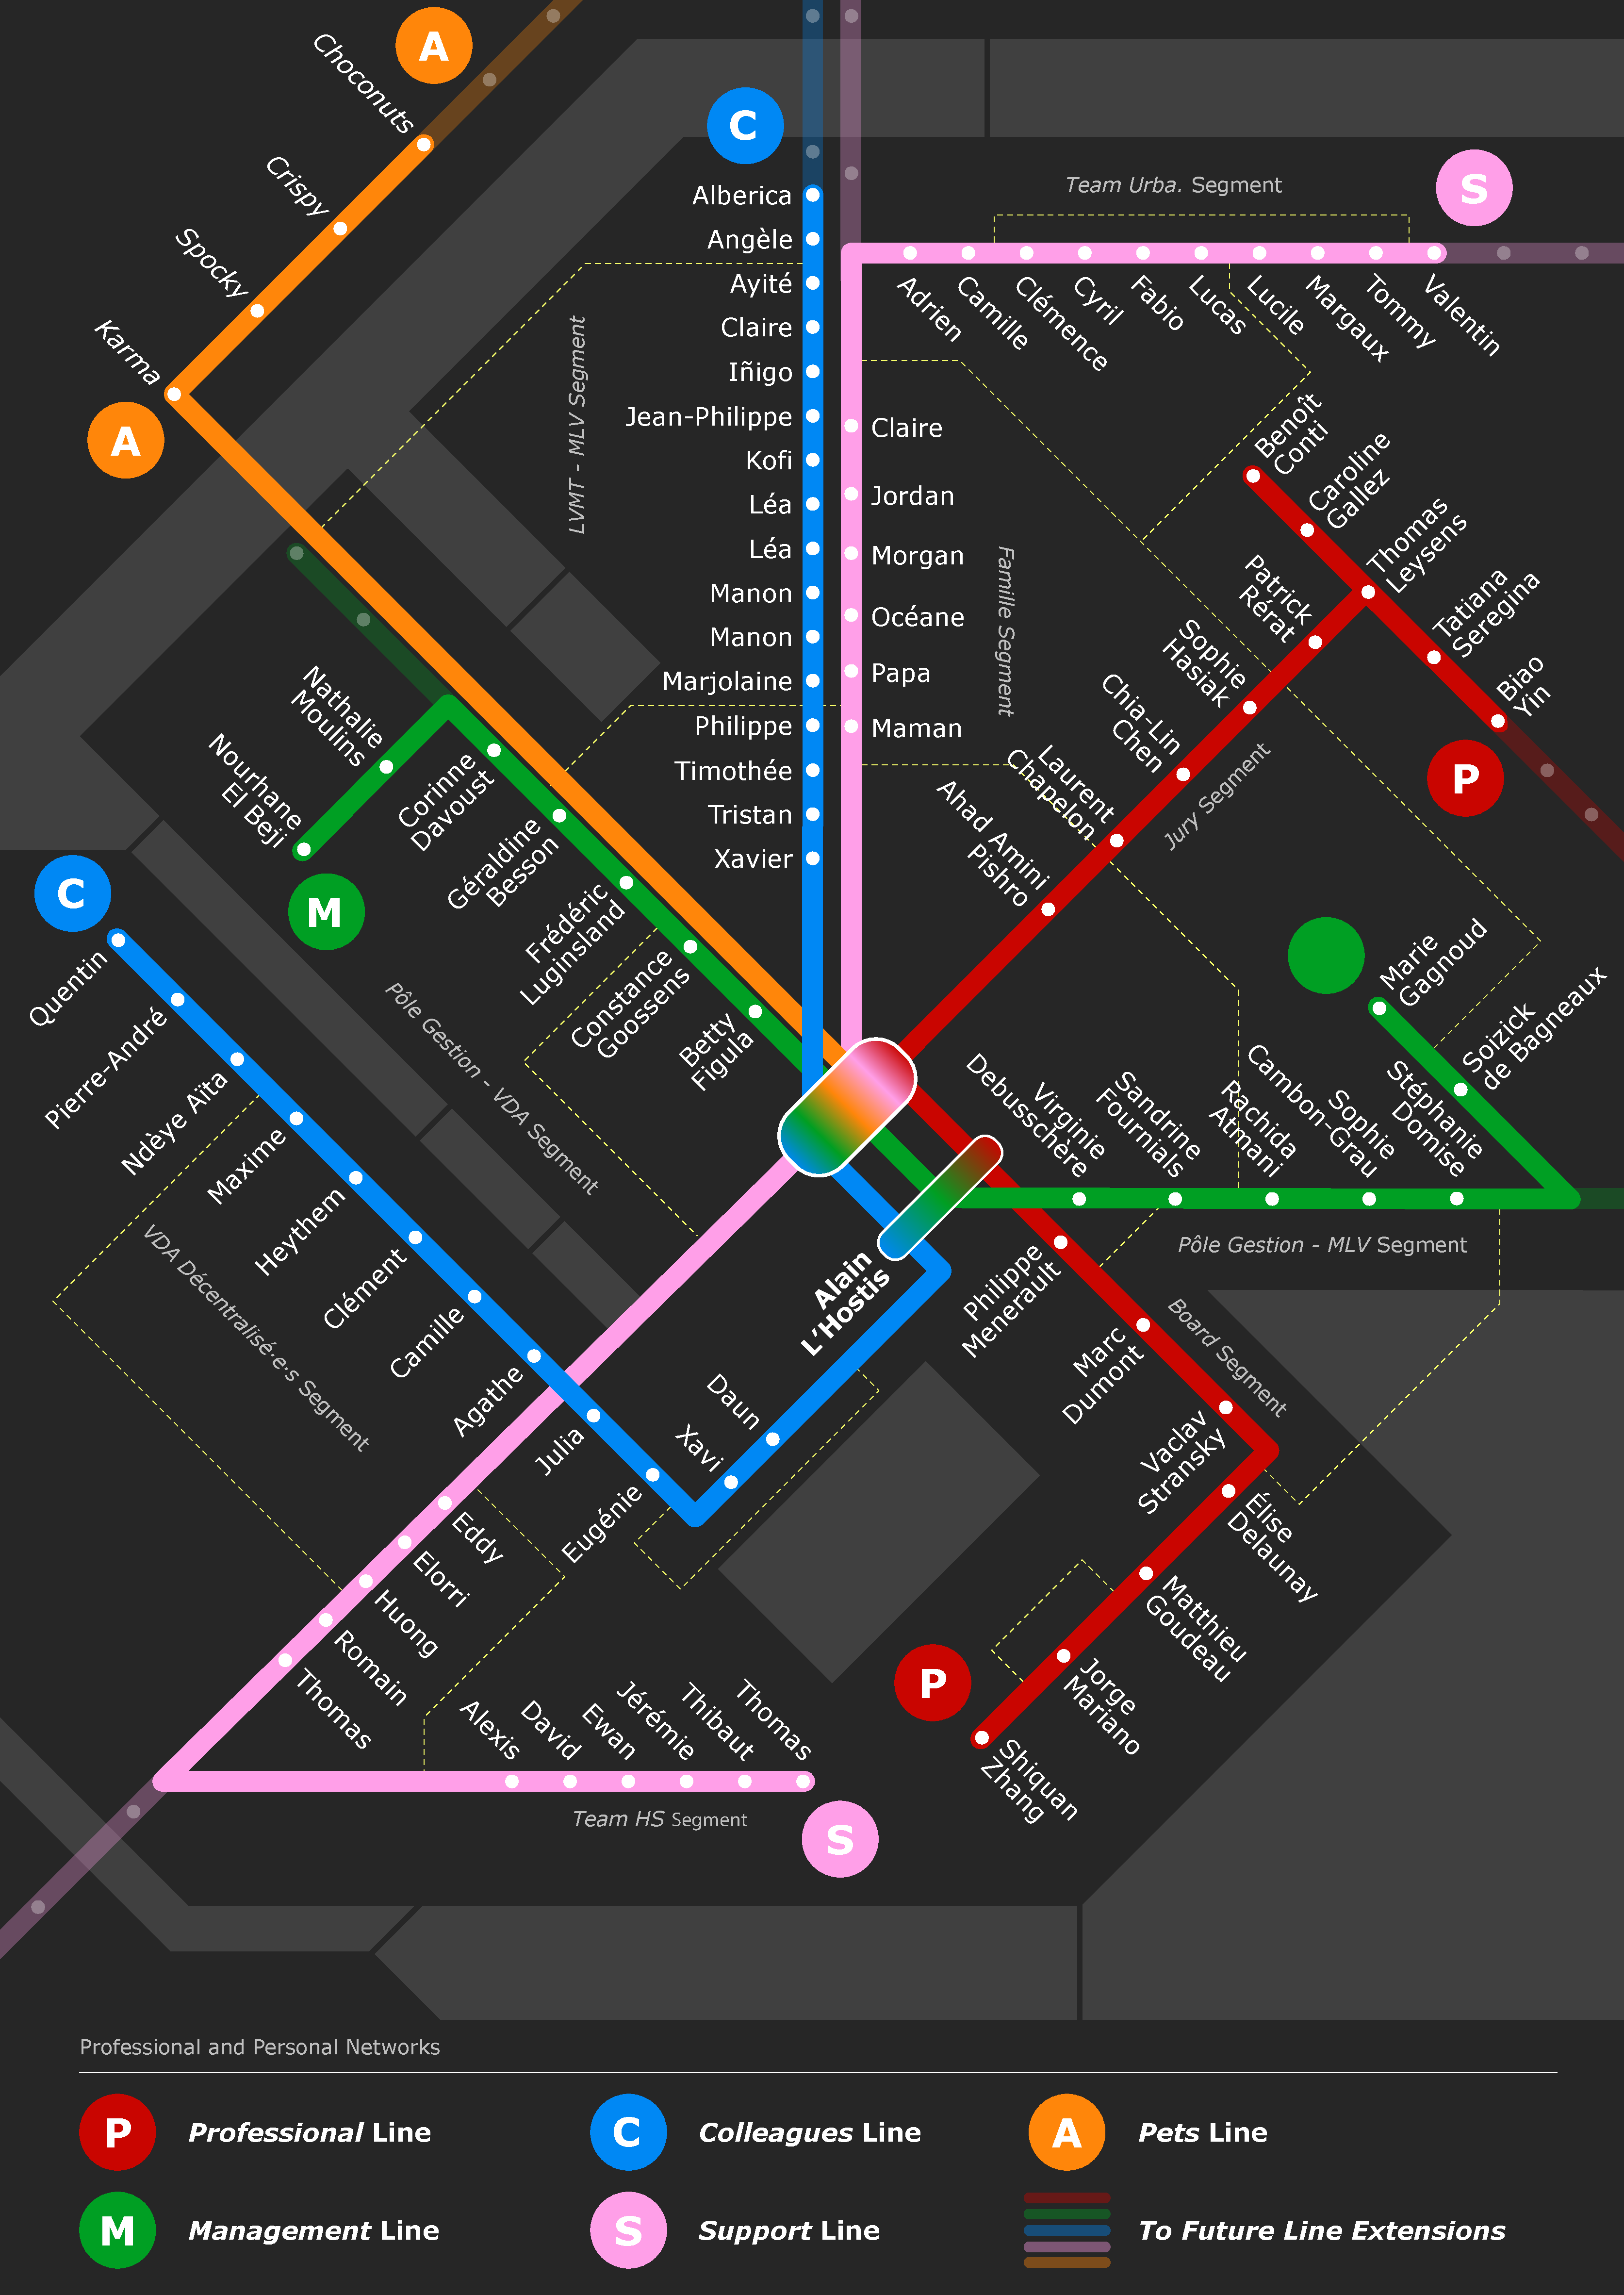
\includegraphics[width=1\columnwidth]{src/Figures/Preambule/EN_Remerciements.pdf}}
        \vspace{5pt}
        \begin{flushright}\scriptsize{
        Author: \textcolor{blue}{Dylan Moinse (2024)}
        }\end{flushright}
    \end{carte}